\documentclass[12pt]{article}

\usepackage[a4paper, margin=2.5cm]{geometry}

\usepackage{fontspec}

\setmainfont{Georgia}

\usepackage[round,authoryear]{natbib}

\usepackage{booktabs}

\usepackage{graphicx}

\setlength{\parindent}{0pt}

\setlength{\parskip}{6pt plus 2pt minus 1pt}



% Running margin label

\usepackage[useregional]{datetime2}

\usepackage{eso-pic}

\newcommand{\mymarginlabel}{\textcopyright\ 2026 David Ewing dew59@uclive.ac.nz | \DTMnow\ | \jobname.tex}



\title{Tweet Sentiment Label Quality: A Text Classification Analysis}

\author{David Ewing · Student ID: 82171165}

\date{}



\begin{document}

\maketitle

\section*{1 Problem Statement}



This project examines how well an automated text classifier can reproduce the sentiment labels applied to a large sample of tweets. The dataset---Cardiff NLP's tweet\_eval sentiment subset---has 45,615 tweets, each tagged as negative, neutral, or positive. Labelling was conducted as part of the SemEval 2017 Task 4A shared task on sentiment analysis in Twitter \citep{rosenthal2017semeval}, and the labels are widely used as an NLP benchmark.

My central questions: 

\begin{itemize}
  \item \textit{How reliably is a text classifier able to reproduce the human-assigned sentiment labels?}
  \item \textit{What does a text classifier's performance tell us about the quality and consistency of the labels?}
\end{itemize}

This matters because  classification performance may reflect  the difficulty of the task and inconsistency in how the labels were assigned. 
A classifier that struggles on neutral tweets may be picking up that the boundary
between neutral and mildly positive or mildly negative is genuinely ambiguous.
Different annotators may draw the line differently,
 e.g, low F1 may be evidence of noisy labels. Both may be true at once.

Four smaller questions guide this analysis:

\begin{enumerate}

  \item What kinds of problems are present in the labelling of tweets?

  \item What types of tweets are systematically hard to classify?

  \item What features are most helpful for distinguishing sentiment classes?

  \item Does removing the neutral class substantially improve classifier performance?

\end{enumerate}

Annotated datasets are expensive to produce. 
My assumption ---
 once created it is used repeatedly. 
 Models comparisons will be using the same labels, and not be questioned. 
 Gold-standard labels  then contain systematic noise. 
Model comparison to a benchmark then includes this systematic noise. 
 
 A model with a higher F1 than a competitor may then
 be better at reproducing the particular pattern 
 of annotator disagreement. 
 I think being explicit about label quality matters.

Macro average F1 is the most appropriate metric for this task. 
The validation split has 2,000 tweets. 
The training data has a class-imbalanced---neutral tweets make up about 45\%. 
To address this, random undersampling was applied to reduce all classes to the size of the smallest. Every class ends up with 7,093 tweets---so 21,279 in total. 
I did not want to oversample.
A model that simply memorises or recombines training examples would be a bad fit.
The training data already has noisy or unreliable labels. 
Learning to replicate those examples would just bake the noise in rather than generalise past it



\section*{2 Dataset}



The dataset is the sentiment subset of the Cardiff NLP tweet\_eval benchmark \citep{barbieri2020tweeteval}, collected from Twitter and annotated for the SemEval 2017 Task 4A competition.
Labels---negative, neutral, and positive---were assigned by crowdsourced annotators, with the final label determined by majority vote.
I find myself questioning whether majority vote is really an adequate basis for a gold standard.
It is cost-effective, but it introduces noise that is difficult to separate from genuine disagreement.

The labels came from Amazon Mechanical Turk\footnote{Amazon Mechanical Turk (MTurk) is a crowdsourcing platform where requesters post small tasks and workers complete them for small payments, typically a few cents each.}.
Workers were paid small amounts to read each tweet and click a sentiment label \citep{rosenthal2017semeval}.
No expertise required.
Each tweet receives at least three annotations.
The majority label stands.
Annotators disagree---sometimes the final label reflects little more than a coin toss---and when I look at the data closely, the so-called ``ground truth'' starts to feel less certain:

\begin{itemize}

  \item a mildly sarcastic tweet;

  \item an expression of resignation that could be read as neutral or mildly negative; and

  \item the resulting label may not reflect genuine consensus.

\end{itemize}

  If a model gets a tweet ``wrong'', I can't help but ask if the gold label was ever solid to begin with.
  A lot of times, it wasn't.

Random undersampling (random\_state=82171165) was applied to balance the training classes, producing 21,279 tweets---7,093 per class.
The validation split (2,000 tweets) serves as the evaluation set throughout.
The test split (12,284 tweets) is held out and not used.
Exact per-class counts at each stage are shown in notebook section 2.5.

The validation set is class-imbalanced: 312 negative, 869 neutral, 819 positive.
The negative class has fewer than half the examples of positive, and less than 40\% as many as neutral.
The moment I noticed this, I realised that interpreting negative-class results would require care.
Poor performance there could reflect label noise, weak feature representations, or simply insufficient test examples---most likely some combination of all three.

A further complication is that confidence intervals for per-class estimates differ substantially.
With only 312 negative tweets, any F1 score for that class carries wide error bars compared to the 869 neutral examples.
When I observe a gap between negative and neutral F1, I cannot be confident whether it reflects a genuine difference or sampling noise.
The difference cannot be ignored, but it should not be overstated.

Tweets are short, informal, and noisy: hashtags, @-mentions, URLs, slang, emoji, and abbreviations are common. They are also highly context-dependent. The same words can carry different sentiments depending on:

\begin{itemize}

  \item the event being discussed;

  \item who is being addressed; and

  \item whether the author is being ironic.

\end{itemize} Tweets about a sports loss sometimes use ``great'' sarcastically---I found several such examples when reviewing the data. Others, directed at celebrities, use ``love'' sincerely. These properties make Twitter sentiment harder to classify reliably than product reviews or news text, where context is more stable and language use more predictable. I did not run a systematic comparison, but the informal evidence from manual review supports this view.

I reviewed a random sample of 10 training tweets during the exploratory phase. Many were genuinely ambiguous even on careful reading. One: a concert announcement in entirely neutral descriptive language, labelled positive. This is defensible---the author clearly approved of the event---but the text alone gives no obvious signal. Another expressed mild frustration indirectly---no swearing, no exclamation, just a brief complaint---and was labelled neutral. I would have called it negative. These borderline cases are prevalent in Twitter data, and I expect the classifier to struggle with them for the same reasons a careful human reader might pause.



\section*{3 Model}



Given the pipeline's modular feature assembly and the need for interpretable baselines, I chose to run these two classifiers,
\begin{itemize}
  \item logistic regression, and
  \item a shallow decision tree,
\end{itemize}
across six feature setups and two task types. That makes four total runs. Both use the same scikit-learn pipeline, balanced training, and I  check performance on the validation split. Figure 1 in the notebook shows the pipeline.

The pipeline operates as follows:
\begin{itemize}
  \item TextCleaner normalises whitespace;
  \item SpacyPreprocessor tokenises each tweet using the \texttt{en\_core\_web\_sm} spaCy model and caches the results in an SQLite feature store;
  \item FeatureUnion assembles the feature matrix from the active feature blocks; and
  \item the classifier receives the matrix and generates predictions.
\end{itemize}
Swapping feature configurations is straightforward---preprocessing remains constant across all runs.

The classifiers are configured as follows:

{\leftskip=1.5em
\begin{tabular}{@{\textbullet\quad}llll@{}}
logistic regression: & \texttt{max\_iter}  & \texttt{= 5000,} & \texttt{random\_state = 82171165;} \\
decision tree:       & \texttt{max\_depth} & \texttt{= 3,}    & \texttt{random\_state = 82171165.} \\
\end{tabular}\par}
That shallow depth means no more than seven leaf nodes,

\begin{itemize}

  \item it is forced to identify only the most discriminating features;

  \item the resulting model is 
  small enough to visualise; and

  \item small enough to interpret directly.

\end{itemize}

I made the tree shallow on purpose.
I wanted to understand what the model latches onto more than getting the highest score.
The \texttt{max\_depth=3} setting is as much a diagnostic tool as a classifier (see Section 5).



\subsection*{3.1 Feature configurations}



Six feature configurations are tested. They are designed to progress from simple token-count representations through to richer, more linguistically informed features, so that each step in complexity can be assessed against the baseline.

\textbf{Unigrams.} A TokensVectorizer extracts count features for the top 200 unigrams, after removing stop words and punctuation, with lowercasing applied. This is the simplest possible bag-of-words representation---word order, negation, and context are all discarded. I expected this to perform poorly, and it does to some degree. Still, it gives me a floor --- anything worse than this is a real problem.

\textbf{Bigrams.} The same vectorizer extracts the top 200 most frequent bigrams. Bigrams capture some local context---``not good'' differs from ``good''---but remain shallow and sensitive to data sparsity. Twitter language is highly varied. Most bigrams are rare. A bigram like ``really love'' may appear frequently, but ``really enjoy'' or ``absolutely love'' might appear only once. The top-200 constraint captures only the most common patterns, which are not always the most sentiment-informative.

\textbf{Unigrams with POS tags (uni+pos).} A FeatureUnion combines the top 100 unigram counts (scaled) with POS tag sequence features from a POSVectorizer. The motivation is that grammatical structure may carry sentiment signal that vocabulary alone misses---intensifiers, negations, and adjective usage patterns may be partially captured here. Negation is a known failure mode for bag-of-words models: ``not'' flips the sentiment of whatever follows, but a unigram model treats the two tokens as independent. POS tags do not fully resolve this, but they add structural information that may help at the margins.

\textbf{Text statistics (textstats).} A TextstatsTransformer extracts surface-level features---tweet length, punctuation counts, and similar properties---scaled with StandardScaler. Negative tweets tend to use more punctuation and exclamation marks. Short tweets are often reactive expressions. Longer ones tend toward neutral, more analytical content. I doubted textstats would perform well in isolation but expected it might contribute in combination with other features. I ran it alone mainly to see what surface properties could do on their own.

\textbf{VADER lexicon (lexicon).} A LexiconCountVectorizer counts matches against the VADER sentiment lexicon, scaled with StandardScaler. VADER was designed specifically for social media sentiment \citep{hutto2014vader}:

\begin{itemize}

  \item it encodes human judgements about which words are positive, negative, and neutral;

  \item it includes common social media expressions; and

  \item it includes emoticons and slang.

\end{itemize} This is probably the most directly relevant feature set for this task. I expected it to perform well. The key question is whether the lexicon covers enough of the actual vocabulary in the tweet\_eval dataset, which was collected later than the original VADER development set.

\textbf{Embeddings.} A Model2VecEmbedder generates dense vector representations of each tweet using a pre-trained embedding model. Embeddings capture semantic similarity in ways that sparse count features cannot---two tweets expressing the same sentiment in different words should produce similar vectors. Whether this generalises to short, noisy Twitter text is an open question. Pre-trained embeddings reflect the distributional properties of their training corpus; if that corpus is general-purpose text rather than social media, the embeddings may not reliably represent informal, abbreviated Twitter language. Of everything I tested, the embeddings gave me the most to think about.



\subsection*{3.2 Task variants}



The 3-class task (negative, neutral, positive) is the primary task. The binary task (negative vs positive only, with neutral tweets excluded) was more of a diagnostic run. My instinct was to start with the simpler binary task and then ask what happens when neutral is added back. Here's the idea: if performance jumps substantially in the binary setting, then the trouble is concentrated at the neutral boundary. If not, the mess is spread somewhere else. That's directly relevant to sub-question 4.

For the binary task, a separate, independently undersampled training and test split was constructed. The binary training set contains 14,186 tweets (7,093 per class), and the binary test set contains 1,131 tweets.



\section*{4 Results}



The results are organised into four runs:

\begin{itemize}

  \item RUN 3: binary $\times$ logistic regression;

  \item RUN 4: binary $\times$ decision tree;

  \item RUN 1: 3-class $\times$ logistic regression;

  \item RUN 2: 3-class $\times$ decision tree.

\end{itemize} The binary runs are presented first to establish a cleaner baseline: without the neutral class, the classification boundary is simpler and the results are easier to interpret. The 3-class runs follow, where the added complexity of neutral reveals the primary sources of difficulty. For each run, classification reports and confusion matrices are shown for all six feature configurations. A summary table and a 3-class vs binary comparison table are provided at the end of this section.



\subsection*{4.1 RUN 3 and RUN 4: binary task}



In the binary task, neutral tweets were excluded and the classifier was asked to distinguish negative from positive only. If all the trouble was really concentrated at the neutral boundary, this should make things a lot easier. I expected a significant gain.

The gain table at the end of Section 4 shows how macro F1 changes from 3-class to binary for each feature configuration. A large positive gain for most configurations would confirm that neutral is the primary source of difficulty. A small or inconsistent gain would suggest that the negative--positive boundary is also problematic, possibly because of label inconsistency at both boundaries.

The decision tree acts differently in the binary setting. Without the neutral class as a majority-class anchor, the tree must find a split that distinguishes negative from positive. This could mean a more useful model---maybe recall balances out more. Or maybe it just shifts which class gets over-predicted. Depends on the features. This is one of the results I was most curious to see.



\subsection*{4.2 RUN 1: 3-class classification, logistic regression}



The classification reports and confusion matrices for RUN 1 cover all six feature configurations. The unigram baseline achieved a macro F1 of 0.447, which serves as the reference point for all subsequent configurations. I was initially surprised that raw word counts performed this well---words like ``love'', ``hate'', ``great'', and ``terrible'' appear in the top 200 and carry clear sentiment signal. The model is doing something real. For a random three-class guesser, macro F1 would be 0.333. We are well above that.

The unigram model cannot handle negation, context, or words that appear across multiple sentiment classes. Terms like ``day'', ``time'', and ``people'' appear frequently in both positive and negative tweets and receive near-zero weights. The model relies on a small set of vocabulary items reliably associated with a single class. This is acceptable as a baseline, but it leaves a great deal unexplained.

VADER lexicon was built for this job. It bakes in how people judge sentiment words and grabs social-media slang you won't find in old-school vocabulary lists. I expected it to outperform the unigram baseline, and the results are worth looking at closely when assessing which feature type captures the most useful signal. If it only boosts negative precision, maybe it's just good for spotting strong negative language and not much else.

Embeddings are supposed to be the most semantically rich. In theory, they grab meaning beyond just counting words. But do they actually do better on noisy, short tweets? That's a real question, and the answer from this dataset says a lot about the limits of general-purpose semantic representations.

\begin{figure}[h]
\centering
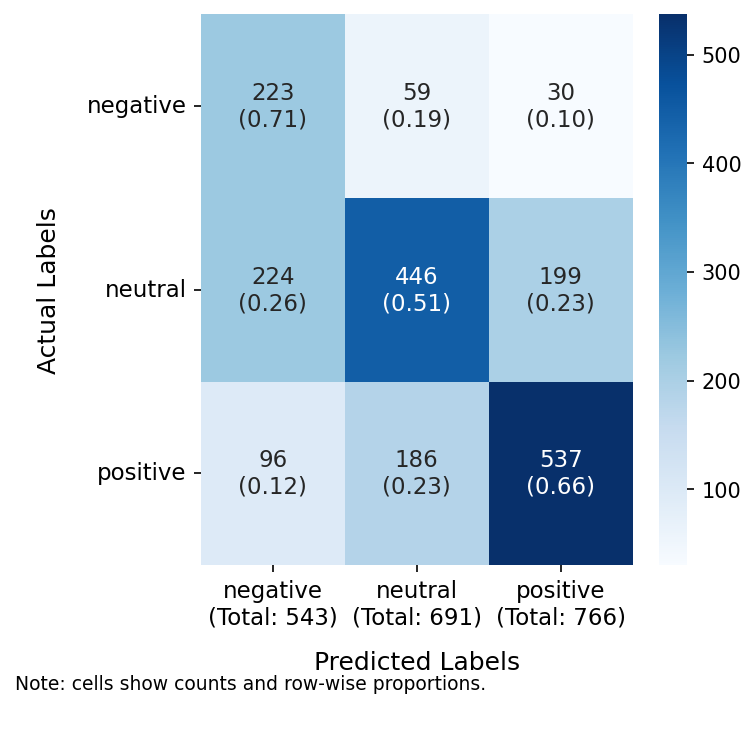
\includegraphics[width=0.7\textwidth]{media/cm_run1_embeddings_LR.png}
\caption{Confusion matrix: 3-class logistic regression with embeddings (macro F1 = 0.590). Errors spread realistically across all three classes --- the model is genuinely uncertain, not just defaulting to neutral.}
\label{fig:cm_lr_embeddings}
\end{figure}



\subsection*{4.3 RUN 2: 3-class classification, decision tree}



The decision tree performed substantially worse than logistic regression across most feature configurations. With unigram features and max\_depth=3, its macro F1 was 0.277---barely above the 0.333 floor of random chance. It predominantly predicts neutral for most inputs. Recall for neutral approaches 1.0, while recall for negative and positive is near zero. This is consistent with shallow tree behaviour: ``predict the most common class'' is the least-bad rule when only three splits are available.

But it's not just weaker---it fails in a totally different way. Logistic regression spreads its mistakes around. The tree just gives up and uses a near-trivial heuristic. Three levels deep isn't enough for anything subtle. Maybe the features just don't offer clean single-variable splits, either. Sentiment isn't a simple threshold on one word count.

Accuracy for the tree? 0.474. Logistic regression? 0.470. Practically the same. But this is exactly why accuracy is the wrong metric for imbalanced multi-class problems. You can overwhelmingly predict the majority class and look fine on paper, but you're useless for the others. Macro F1 catches this; accuracy hides it. Running both models side by side on this dataset taught me more than any textbook example.

\begin{figure}[h]
\centering
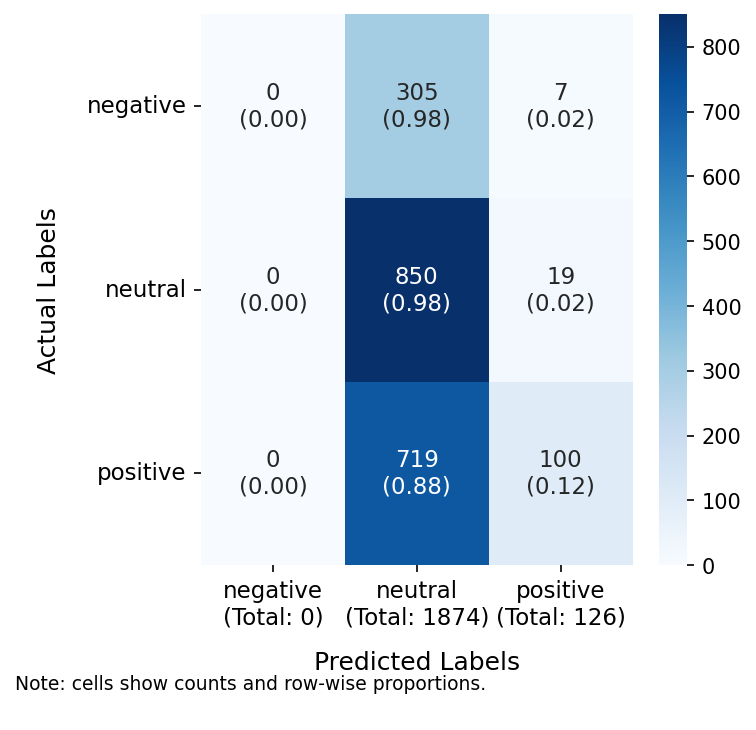
\includegraphics[width=0.7\textwidth]{media/cm_run2_unigrams_DT.png}
\caption{Confusion matrix: 3-class decision tree with unigrams (macro F1 = 0.277). The tree predicts neutral for almost every input --- recall for negative and positive is near zero.}
\label{fig:cm_dt_unigrams}
\end{figure}



\subsection*{4.4 3-class vs binary: gain summary}



\begin{table}[h]
\centering
\caption{Macro F1 for 3-class and binary tasks, and gain from removing neutral.}
\label{tab:gain}
\small
\begin{tabular}{lrrr@{\hspace{2em}}rrr}
\toprule
& \multicolumn{3}{c}{Logistic Regression} & \multicolumn{3}{c}{Decision Tree} \\
\cmidrule(lr){2-4} \cmidrule(lr){5-7}
Feature set & 3-class & binary & gain & 3-class & binary & gain \\
\midrule
unigrams   & 0.466 & 0.667 & +0.201 & 0.277 & 0.521 & +0.244 \\
bigrams    & 0.335 & 0.525 & +0.190 & 0.232 & 0.448 & +0.217 \\
uni+pos    & 0.472 & 0.650 & +0.178 & 0.327 & 0.561 & +0.234 \\
textstats  & 0.387 & 0.540 & +0.154 & 0.369 & 0.553 & +0.184 \\
lexicon    & 0.540 & 0.639 & +0.099 & 0.539 & 0.638 & +0.098 \\
embeddings & 0.590 & 0.806 & +0.216 & 0.419 & 0.614 & +0.195 \\
\bottomrule
\end{tabular}
\end{table}



\section*{5 Discussion}



\subsection*{5.1 Overall performance}



The logistic regression baseline achieved a macro F1 of 0.447 on the 3-class task.  
A score below 0.5 is not strong, but it is not meaningless .  
With the level of annotation noise present and the known difficulty of the neutral class, a macro F1 in the 0.4--0.5 range is a credible baseline.
A random classifier on a balanced three-class problem would achieve macro F1 of 0.333. 
A model that always predicts the majority class gets high recall for one class but near-zero for the rest---macro F1 drops below 0.333. So 0.447 from logistic regression is comfortably above both floors. The real question isn't whether the classifier works at all. It's why it doesn't work better, and what that says about the data.

The decision tree's macro F1 was 0.277---tough to defend. Accuracy? 0.474, basically the same as logistic regression (0.470). That just shows how useless accuracy is here. With 43.5\% neutral in the test set, a model can just say ``neutral'' for every input and score 43.5\% accuracy without learning anything. The tree isn't quite that bad, but it's close. Macro F1 exposes this; accuracy conceals it.



\subsection*{5.2 Feature comparison}



The six feature configurations produced different results, and a few patterns stood out.
I started with unigrams as the baseline, from the lab work, Bigrams seemed like a natural extension, 
though I suspected Twitter's noisy, varied vocabulary might limit how much local context they actually captured.
Adding POS tags felt like it would help by introducing  grammatical structure.
Text statistics were the most speculative---things like tweet length and punctuation density felt like blunt proxies for emotional intensity,
 and I wasn't confident they'd contribute much on their own.
VADER I felt better about.
Embeddings I was less certain about going in.

As I said, I thought the VADER lexicon might do the best.
It was designed for social media, encodes human judgements about sentiment, and incorporates slang, emoticons, and expressions that general vocabulary counts miss.
\citet{hutto2014vader} showed it worked well on Twitter data, and this task felt very close to what they evaluated it on.


If the embeddings came from generic text rather than social media, I expected they'd struggle with the informal shorthand.
A tweet like ``can't even rn'' expresses frustration, but I wasn't confident a general-purpose embedding model would reliably encode it as negative.

I wasn't sure whether text statistics would contribute anything useful.
Tweet length, punctuation count, capitalisation patterns---these feel like blunt proxies for emotional intensity, and I wasn't confident there was real signal there.
I figured short tweets are often reactive, and heavy punctuation might signal strong emotion---but that's a guess.
I ran them as a standalone configuration mainly to see what they'd actually do on their own, rather than having them buried inside a combined model where their contribution would be invisible.

One pattern I noticed when comparing feature configurations: the per-class ordering remains  stable.
In logistic regression, per-class F1 almost always follows negative $<$ positive $<$ neutral, even as the absolute values vary.
I believe this suggests the relative difficulty of each class is a property of the data rather than any particular feature representation.
The negative class is harder to classify regardless of the features used---that is a data observation, not a modelling one.



\subsection*{5.3 What the binary task reveals}



Sub-question 4 is really asking: was neutral the problem all along, or is the trouble more general? 

If dropping neutral produces a large, consistent improvement across classifiers and feature types, that would suggest neutral was the main source of difficulty---a middle category that's  hard to separate from mild negative and mild positive expression.
That would fit with what I'd read about the SemEval annotation process, where neutral was the default label for tweets that didn't clearly go one way or the other.

But if the gain is small or inconsistent, it suggests the difficulty isn't just at the neutral boundary.
Maybe the negative--positive boundary is also messy, or the features just aren't rich enough to resolve it regardless.
I found this the more interesting possibility, honestly.

Table~\ref{tab:gain} shows macro F1 for both setups and the gain from dropping neutral.
I found that view more useful than raw F1 figures---it speaks directly to where the difficulty is concentrated rather than just how well the model did overall.
Big, consistent gains would suggest neutral is mostly to blame.
Small or variable gains would suggest the problem is spread more evenly.

The binary task uses a different, smaller test set---the validation set with all neutral tweets removed.
So some of any F1 gain might just reflect the changed composition rather than the task being genuinely easier.
I don't think it reverses the picture, but it complicates a clean comparison.



\subsection*{5.4 Class-level analysis}



The 3-class LR results are not balanced across classes.
Positive tweets got the best F1, with high precision but only middling recall---the model doesn't call many tweets positive, but when it does, it's usually right.
negative is the worst performer: low precision, moderate recall.
The model tags too many tweets as negative, and most of those turn out to be neutral or positive.
Neutral sits in the middle.

I didn't expect neutral to beat negative, but it did.
The conventional view---supported by the course notes and by \citet{kenyondean2018sentiment}---is that neutral is the hardest class because it lacks distinctive lexical markers.
The results don't clearly support this.
Neutral F1 exceeds negative F1.
Maybe that's because neutral is the largest group in the test set, giving the model more evaluation signal.
Or maybe neutral tweets genuinely cluster around non-sentiment-loaded vocabulary that shows up well in the top-200 unigrams.
negative might just be more varied and context-dependent language-wise.

The decision tree collapse is a separate phenomenon.
It's not just weak on negative and positive---it's nearly zero on both.
The tree has apparently learned that predicting neutral minimises loss on the training data even after undersampling.
That bothers me.
It suggests the feature representations don't yield a clean split between neutral and the other classes at any single threshold.



\subsection*{5.5 Label quality evidence}



The thing I kept returning to is that a low macro F1 doesn't tell you much on its own.
It could be the features, the model, the labels, or all three.
All three are probably true to some degree here, and I genuinely cannot tell which dominates.

negative stands out. Low precision means the model generates many false positive predictions for negative sentiment. If the model predicts negative based on reasonable lexical cues but the gold label is neutral, this suggests annotators labelled borderline tweets as neutral rather than negative. The SemEval annotation guidelines used neutral as the default for tweets that did not clearly express positive or negative sentiment. The neutral label may have introduced systematic ambiguity in this dataset \citep{kenyondean2018sentiment}:

\begin{itemize}

  \item the category was designed to capture genuine neutrality alongside mild negative expression;

  \item annotators were uncertain about tweets that fell between the two;

  \item sentiment is a property of the author's relationship to content, not just of the words used.

\end{itemize}

A phrase like ``not bad at all'' could be positive or ironic depending on context. Unigram count features, which discard word order, negation scope, and context, are poorly equipped to capture these distinctions. But sometimes, the trouble isn't the model's fault---it's just genuinely ambiguous:

\begin{itemize}

  \item even human annotators would disagree on these cases;

  \item the low classifier performance may be tracking that annotator disagreement;

  \item rather than merely reflecting model inadequacy.

\end{itemize}

I kept coming back to the negative precision.
It's low, but not in a random way.
The model and the annotators seem to agree that certain vocabulary is negative, but their labels keep diverging:

\begin{itemize}

  \item the model predicts negative, and in many cases the tweet probably is negative in some sense;

  \item the annotators, however, labelled it neutral;

  \item possibly because the expression was not strong enough to trigger the positive or negative label.

\end{itemize} If I had access to per-annotator votes rather than only the majority-vote outcome, I could check whether these tweets had high disagreement rates. Not having that is a genuine limitation.



\subsection*{5.6 Misclassification analysis}



I ran the misclassification breakdown in notebook section 4.2.
Looking at individual cases where the model went wrong felt more useful than just staring at the summary F1.

Some misclassifications are model failures. A tweet containing strongly negative language predicted as neutral is likely a case where the relevant tokens fell outside the top-200 vocabulary, or where negation flipped the meaning of otherwise neutral words. These are feature engineering problems.

Other misclassifications are more interesting. When I checked tweets the model called negative but the label was neutral, a recurring pattern came up:

\begin{itemize}

  \item tweets expressing mild dissatisfaction, slight frustration, or low-key complaint;

  \item the kind of expression that sits at the boundary between neutral and negative in everyday language.

\end{itemize} I'd expect human annotators to disagree on these. The model isn't clearly wrong. The label isn't clearly right. That ambiguity is the point.

The same goes for tweets the model calls positive but the label is neutral. Sometimes there's quiet enthusiasm, but the annotator read it as reporting rather than feeling. These borderline cases are exactly what the central research question is about.

Across all feature configurations, the tweets the model consistently misses are the sarcastic, ironic, or highly context-dependent ones. ``Great job guys'' directed at a losing team could mean anything. No unigram or bigram feature set can resolve this. A human with knowledge of the team and the result would get it immediately. The classifier has only the words. That's a hard ceiling for surface-form features, and it's a real constraint.

I don't think that's the model's fault, exactly. That just seems to be what this problem is. Did annotators have the context they needed when labelling? If they saw tweets in isolation---no thread, no event background---they probably defaulted to neutral when unsure. That would explain a lot of the patterns observed here.



\subsection*{5.7 Limitations and future directions}



There are things I couldn't do, or wish I'd done differently.

The feature configurations tested here are all applied independently. No multi-feature combinations are evaluated. A combined model may outperform any single configuration:

\begin{itemize}

  \item for example, unigrams plus VADER lexicon plus text statistics;

  \item the interaction effects between feature types are not captured here.

\end{itemize} Mixing features is the obvious next step, and the pipeline architecture supports it directly through FeatureUnion. The cost is missing those interactions; the benefit is a clean additive comparison of what each feature type contributes.

I set max\_depth=3 deliberately --- I wanted to see the actual splits, not just get the highest score.
A deeper tree would likely do better on F1, but I'd lose the ability to read it.
There's a real risk of overfitting too, given the training set size.

The embeddings used here are from a pre-trained general-purpose model. Fine-tuning on Twitter data, or using something like BERTweet (pre-trained on 850 million tweets), would likely produce more useful tweet embeddings. General models just don't always capture the quirks of short, informal text.

The analysis is constrained to the validation split. The held-out test split (12,284 tweets) has not been used and would provide a more reliable estimate of generalisation performance. The validation set has only 312 negative examples, which limits the precision of per-class estimates for that class. Those wide confidence intervals mean negative F1 should be taken as indicative rather than definitive.

The labels themselves are uncertain in ways I can't fix. They're majority-vote outcomes, not ground truth. Where annotators disagreed, the label is uncertain, and classifier performance on those cases is not a reliable measure of model quality. If I had inter-annotator agreement scores, I could separate the genuinely hard cases from the clearly labelled ones. Without that, I cannot distinguish ``model failure'' from ``genuinely contested annotation.'' That is probably the single most valuable extension of this analysis.



\nocite{*}

\bibliographystyle{apalike}

\bibliography{refs}

\appendix

\section{How to Run the Submission Package}

This submission is intended to be distributed as a zip archive.
When unpacking the archive, the top-level folder \texttt{FINAL-PROJECT/} should be kept intact.
The notebook itself should remain inside \texttt{FINAL-PROJECT/python/*.ipynb} and should be opened from that location rather than being moved elsewhere.

For one-line execution after extraction, run \texttt{python run\_submission.py} from the package root.
This launcher executes the notebook via Jupyter \texttt{nbconvert}.

This is important because the notebook uses relative paths and expects enough headroom under \texttt{FINAL-PROJECT/} to create and use sibling folders such as \texttt{data/}, \texttt{figs/}, \texttt{results/}, and \texttt{report/}.
If the folder structure is preserved, no extra setup instructions should be needed by the user.
After the first run has created these working folders, the notebook can also be run manually in the usual way, provided it remains in the same \texttt{FINAL-PROJECT/python/} location.

\begin{verbatim}
  python -m zipfile -e FINAL-PROJECT-SUBMISSION.zip .
  python run_submission.py
\end{verbatim}

\end{document}
